\documentclass[a4paper]{tp}
\usepackage{tikz}  
\usetikzlibrary{decorations.pathreplacing}
\usetikzlibrary{decorations.markings}
\usetikzlibrary{patterns}
\usetikzlibrary{arrows.meta}
\titre{TP2 : Focométrie}
\begin{document}

\section{Reconnaissance rapide des lentilles}%
\label{sec:reconnaissance_rapide_des_lentilles}
\begin{itemize}
  \item Pour reconnaitre une lentille, on peut commencer par observer sa forme, les lentilles convergentes ont un bord fin alors que les lentilles divergentes ont un bord épais.


\item On peut également observer un objet proche à travers la lentille. En vous appuyant sur des schémas, montrer qu'une lentille convergente forme d'un objet proche une image agrandie alors que l'image formée par une lentille divergente d'un objet proche est plus petite que l'objet.

\item Si on observe un objet lointain (à l'infini) le critère de distinction est différent. En vous appuyant sur des schémas, montrer que l'image d'un objet lointain par une lentille convergente est retournée alors que celle donnée par une lentille divergente est droite.
\end{itemize}

\section{Lentilles convergentes}%
\label{sec:lentilles_convergentes}

\subsection{Estimation rapide}%
\label{sub:estimation_rapide}

Pour estimer rapidement la distance focale d'une lentille convergente, on peut former l'image d'un objet lointain sur un écran. La distance focale de la lentille est alors la distance entre la lentille et l'écran.

\begin{itemize}
  \item Donner une estimation des distances focales des lentilles à votre disposition en utilisant cette méthode.
\end{itemize}


\subsection{Autocollimation}%

La méthode d'autocollimation consiste à placer un miroir derrière la lentille dont on souhaite mesurer la distance focale. Lorsque l'image de l'objet se trouve dans le même plan que l'objet, celui-ci se trouve dans le plan focal de la lentille.


\label{sub:autocollimation}
\begin{center}
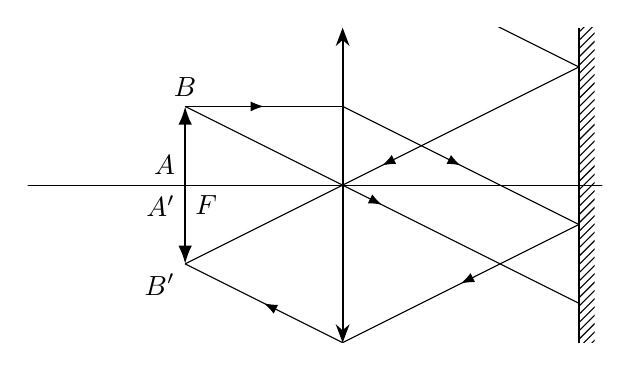
\begin{tikzpicture}[
  rayon/.style = {postaction={decorate},decoration = {markings, mark = at position 0.5 with {\arrow{Latex}}}}
  ]
\path[clip] (1,-2) rectangle (8.3,2);
\draw[->] (0,0) -- (10,0);
\draw[thick,Stealth-Stealth] (5,-2) -- (5,2);
\coordinate (O) at (5,0);
\draw[thick] (8,-2) -- (8,2);
\path[pattern=north east lines] (8,2) rectangle (8.2,-2);
\draw[thick,-Latex] (3,0) coordinate (A) node[below right]{$F$} node[above left]{$A$} -- (3,1) node[above]{$B$} coordinate(B);
\draw[thick,-Latex] (3,0) node[below left]{$A'$}  -- (3,-1) coordinate (Bp) node[below left]{$B'$};
\draw[rayon] (B) -- (B-|O);
\draw[rayon] (5,1) -- (8,-0.5);
\draw[rayon] (8,-0.5) -- (5,-2);
\draw[rayon] (5,-2) -- (Bp);

\draw[rayon] (5,3) -- (8,1.5);
\draw[rayon] (8,1.5) -- (Bp);
\draw[rayon] (B) -- (8,-1.5);

\end{tikzpicture}

\begin{itemize}
  \item Appliquer la méthode d'autocollimation pour déterminer la distance focale d'une lentille convergente.
\end{itemize}

\end{center}
\subsection{Méthode de Bessel}%
\label{sub:methode_de_bessel}

Lorsqu'on positionne un objet et un écran à une distance $D$ l'un de l'autre, on peut former l'image de l'objet sur l'écran par une lentille convergente de distance focale $f'$  à condition que la relation de conjugaison soit vérifiée. Si on note $p=\ol{OA}$ la distance entre la lentille et l'objet, on peut montrer (le faire ?) que l'image de l'objet sera sur l'écran à condition que 
\begin{equation*}
  D = -\frac{p^2}{p + f'}
\end{equation*}

Lorsqu'on inverse cette équation pour trouver $p$ en fonction de $D$, on trouve que si $D>4f'$ il existe deux solutions :
\begin{equation*}
  p = -\frac{D}{2}\pm \frac{\sqrt{D^2-4Df'}}{2}
\end{equation*}

La distance $d$ entre les deux positions de la lentille donnant une image nette sur l'écran est 
\begin{equation*}
  d = \sqrt{D^2-4Df'} \quad \text{donc} \quad f' = \frac{D^2-d^2}{4D}.
\end{equation*}

\begin{itemize}
  \item En déterminant les deux positions donnant une image nette de l'objet sur l'écran, déterminer $d$ et en déduire la valeur de la distance focale de la lentille.
\end{itemize}

\subsection{Méthode de Silbermann}%
\label{sub:methode_de_silbermann}
C'est un cas particulier de la méthode précédente dans le cas où $D=4f'$. Dans ce cas il n'existe qu'une seule position de la lentille donnant une image nette de l'objet sur l'écran.


\begin{itemize}
  \item Ajuster la distance entre l'objet et l'écran jusqu'à ce qu'il n'y ait plus qu'une seule position de la lentille donnant une image nette de l'objet sur l'écran et en déduire la valeurs de $f'$.
\end{itemize}

\section{Lentilles divergentes}%
\label{sec:lentilles_divergentes}

\subsection{Méthode du doublet accolé}%
\label{sub:methode_du_doublet_accole}

On appelle \emph{doublet accolé} deux lentilles suffisamment proches l'une de l'autre pour que leurs centres optiques puissent être considérés comme confondus. Le système ainsi formé peut être assimilé à une lentille mince dont la vergence est la somme des vergences des deux lentilles minces accolées.

\begin{itemize}
  \item Lorsqu'on colle une lentille convergente de focale $f_1$ et une lentille divergente de focale $f_2$, déterminer la condition sur $f_1$ et $f_2$ pour que le doublet se comporte comme une lentille convergente.

\item Réaliser un doublet accolé convergent en utilisant une lentille convergente de distance focale connue et une lentille divergente dont on veut déterminer la distance focale. Utiliser une des méthodes précédentes pour déterminer la distance focale du doublet et en déduire la distance focale de la lentille divergente. 

\end{itemize}

\end{document}
